% -*- mode: latex; coding: utf-8 -*-

\documentclass[conference]{IEEEtran}

% -*- mode: latex; coding: utf-8 -*-
% *** FONTS ****
%
\DeclareFixedFont{\ttb}{T1}{txtt}{bx}{n}{9} % for bold
\DeclareFixedFont{\ttm}{T1}{txtt}{m}{n}{9}  % for normal

% *** COLOR PACKAGES ***
%
\usepackage[usenames,dvipsnames,svgnames,table]{xcolor}
\definecolor{linkblue}{rgb}{0,0,0.8}       % Standard
\definecolor{darkblue}{rgb}{0,0.08,0.45}   % Dark blue
\definecolor{bfhgrey}{rgb}{0.41,0.49,0.57} % BFH grey
\definecolor{linkcolor}{rgb}{0,0,0}
% \definecolor{Black}{black}
\definecolor{keywords}{rgb}{1,0,0}
\definecolor{red}{rgb}{0.6,0,0}
\definecolor{green}{rgb}{0,0.5,0}
\definecolor{blue}{rgb}{0,0,0.5}
% Syntax colors
\definecolor{syntaxRed}{rgb}{0.6,0,0}
\definecolor{syntaxBlue}{rgb}{0,0,0.5}
\definecolor{syntaxComment}{rgb}{0,0.5,0}
% Background colors
\definecolor{syntaxBackground}{rgb}{0.95, 0.95, 0.95}


% *** COMMANDS ***
%
\newcommand{\NWtarget}[2]{\hypertarget{#1}{#2}}
\newcommand{\NWlink}[2]{\hyperlink{#1}{#2}}
\newcommand{\NWtxtMacroDefBy}{Fragment defined by}
\newcommand{\NWtxtMacroRefIn}{Fragment referenced in}
\newcommand{\NWtxtMacroNoRef}{Fragment never referenced}
\newcommand{\NWtxtDefBy}{Defined by}
\newcommand{\NWtxtRefIn}{Referenced in}
\newcommand{\NWtxtNoRef}{Not referenced}
\newcommand{\NWtxtFileDefBy}{File defined by}
\newcommand{\NWtxtIdentsUsed}{Uses:}
\newcommand{\NWtxtIdentsNotUsed}{Never used}
\newcommand{\NWtxtIdentsDefed}{Defines:}
\newcommand{\NWsep}{${\diamond}$}
\newcommand{\NWnotglobal}{(not defined globally)}
\newcommand{\NWuseHyperlinks}{}
\providecommand\newthought[1]{%
   % \addvspace{1.0\baselineskip plus 0.5ex minus 0.2ex}%
   \noindent\textsc{#1} % small caps text out
}

% *** LISTING PACKAGES ***
%
\usepackage{listings}
% Define a list style for Python programming language
\lstset{language=Python,
    basicstyle=\ttm\ttfamily,
    backgroundcolor = \color{syntaxBackground},
    columns=fullflexible,
    commentstyle=\ttm\color{green},
    emphstyle=\ttb\color{red},
    escapechar=§,
    frame=tlbr,
    framesep=0.2cm,
    framerule=0pt,
    numbers=left,
    numbersep=5pt,                   % how far the line-numbers are from the code
    numberstyle=\tiny\color{gray}, % the style that is used for the line-numbers
    identifierstyle=\ttm\color{black},
    keywordstyle=\ttb\color{blue},
    otherkeywords={self},
    showspaces=false,
    showstringspaces=false,
    showtabs=false,
    tab=\rightarrowfill,
    xleftmargin=0.7cm,
}


% *** CITATION PACKAGES ***
%
%\usepackage{cite}
% cite.sty was written by Donald Arseneau
% V1.6 and later of IEEEtran pre-defines the format of the cite.sty package
% \cite{} output to follow that of the IEEE. Loading the cite package will
% result in citation numbers being automatically sorted and properly
% "compressed/ranged". e.g., [1], [9], [2], [7], [5], [6] without using
% cite.sty will become [1], [2], [5]--[7], [9] using cite.sty. cite.sty's
% \cite will automatically add leading space, if needed. Use cite.sty's
% noadjust option (cite.sty V3.8 and later) if you want to turn this off
% such as if a citation ever needs to be enclosed in parenthesis.
% cite.sty is already installed on most LaTeX systems. Be sure and use
% version 5.0 (2009-03-20) and later if using hyperref.sty.
% The latest version can be obtained at:
% http://www.ctan.org/pkg/cite
% The documentation is contained in the cite.sty file itself.


% *** GRAPHICS RELATED PACKAGES ***
%
\ifCLASSINFOpdf{}
   \usepackage[pdftex]{graphicx}
  % declare the path(s) where your graphic files are
   \graphicspath{{images/}}
  % and their extensions so you won't have to specify these with
  % every instance of \includegraphics
   \DeclareGraphicsExtensions{.pdf,.jpg,.png}
\else
  % or other class option (dvipsone, dvipdf, if not using dvips). graphicx
  % will default to the driver specified in the system graphics.cfg if no
  % driver is specified.
  % \usepackage[dvips]{graphicx}
  % declare the path(s) where your graphic files are
  % \graphicspath{{../eps/}}
  % and their extensions so you won't have to specify these with
  % every instance of \includegraphics
  % \DeclareGraphicsExtensions{.eps}
\fi
% graphicx was written by David Carlisle and Sebastian Rahtz. It is
% required if you want graphics, photos, etc. graphicx.sty is already
% installed on most LaTeX systems. The latest version and documentation
% can be obtained at:
% http://www.ctan.org/pkg/graphicx
% Another good source of documentation is "Using Imported Graphics in
% LaTeX2e" by Keith Reckdahl which can be found at:
% http://www.ctan.org/pkg/epslatex
%
% latex, and pdflatex in dvi mode, support graphics in encapsulated
% postscript (.eps) format. pdflatex in pdf mode supports graphics
% in .pdf, .jpeg, .png and .mps (metapost) formats. Users should ensure
% that all non-photo figures use a vector format (.eps, .pdf, .mps) and
% not a bitmapped formats (.jpeg, .png). The IEEE frowns on bitmapped formats
% which can result in "jaggedy"/blurry rendering of lines and letters as
% well as large increases in file sizes.
%
% You can find documentation about the pdfTeX application at:
% http://www.tug.org/applications/pdftex


% *** MATH PACKAGES ***
%
\usepackage{amsmath}
% A popular package from the American Mathematical Society that provides
% many useful and powerful commands for dealing with mathematics.
%
% Note that the amsmath package sets \interdisplaylinepenalty to 10000
% thus preventing page breaks from occurring within multiline equations. Use:
\interdisplaylinepenalty=2500
% after loading amsmath to restore such page breaks as IEEEtran.cls normally
% does. amsmath.sty is already installed on most LaTeX systems. The latest
% version and documentation can be obtained at:
% http://www.ctan.org/pkg/amsmath


% *** SPECIALIZED LIST PACKAGES ***
%
%\usepackage{algorithmic}
% algorithmic.sty was written by Peter Williams and Rogerio Brito.
% This package provides an algorithmic environment fo describing algorithms.
% You can use the algorithmic environment in-text or within a figure
% environment to provide for a floating algorithm. Do NOT use the algorithm
% floating environment provided by algorithm.sty (by the same authors) or
% algorithm2e.sty (by Christophe Fiorio) as the IEEE does not use dedicated
% algorithm float types and packages that provide these will not provide
% correct IEEE style captions. The latest version and documentation of
% algorithmic.sty can be obtained at:
% http://www.ctan.org/pkg/algorithms
% Also of interest may be the (relatively newer and more customizable)
% algorithmicx.sty package by Szasz Janos:
% http://www.ctan.org/pkg/algorithmicx


% *** ALIGNMENT PACKAGES ***
%
\usepackage{array}
% Frank Mittelbach's and David Carlisle's array.sty patches and improves
% the standard LaTeX2e array and tabular environments to provide better
% appearance and additional user controls. As the default LaTeX2e table
% generation code is lacking to the point of almost being broken with
% respect to the quality of the end results, all users are strongly
% advised to use an enhanced (at the very least that provided by array.sty)
% set of table tools. array.sty is already installed on most systems. The
% latest version and documentation can be obtained at:
% http://www.ctan.org/pkg/array

% IEEEtran contains the IEEEeqnarray family of commands that can be used to
% generate multiline equations as well as matrices, tables, etc., of high
% quality.


% *** SUBFIGURE PACKAGES ***
%\ifCLASSOPTIONcompsoc
%  \usepackage[caption=false,font=normalsize,labelfont=sf,textfont=sf]{subfig}
%\else
%  \usepackage[caption=false,font=footnotesize]{subfig}
%\fi
% subfig.sty, written by Steven Douglas Cochran, is the modern replacement
% for subfigure.sty, the latter of which is no longer maintained and is
% incompatible with some LaTeX packages including fixltx2e. However,
% subfig.sty requires and automatically loads Axel Sommerfeldt's caption.sty
% which will override IEEEtran.cls' handling of captions and this will result
% in non-IEEE style figure/table captions. To prevent this problem, be sure
% and invoke subfig.sty's "caption=false" package option (available since
% subfig.sty version 1.3, 2005/06/28) as this is will preserve IEEEtran.cls
% handling of captions.
% Note that the Computer Society format requires a larger sans serif font
% than the serif footnote size font used in traditional IEEE formatting
% and thus the need to invoke different subfig.sty package options depending
% on whether compsoc mode has been enabled.
%
% The latest version and documentation of subfig.sty can be obtained at:
% http://www.ctan.org/pkg/subfig


% *** FLOAT PACKAGES ***
%
%\usepackage{fixltx2e}
% fixltx2e, the successor to the earlier fix2col.sty, was written by
% Frank Mittelbach and David Carlisle. This package corrects a few problems
% in the LaTeX2e kernel, the most notable of which is that in current
% LaTeX2e releases, the ordering of single and double column floats is not
% guaranteed to be preserved. Thus, an unpatched LaTeX2e can allow a
% single column figure to be placed prior to an earlier double column
% figure.
% Be aware that LaTeX2e kernels dated 2015 and later have fixltx2e.sty's
% corrections already built into the system in which case a warning will
% be issued if an attempt is made to load fixltx2e.sty as it is no longer
% needed.
% The latest version and documentation can be found at:
% http://www.ctan.org/pkg/fixltx2e

%\usepackage{stfloats}
% stfloats.sty was written by Sigitas Tolusis. This package gives LaTeX2e
% the ability to do double column floats at the bottom of the page as well
% as the top. (e.g., "\begin{figure*}[!b]" is not normally possible in
% LaTeX2e). It also provides a command:
%\fnbelowfloat
% to enable the placement of footnotes below bottom floats (the standard
% LaTeX2e kernel puts them above bottom floats). This is an invasive package
% which rewrites many portions of the LaTeX2e float routines. It may not work
% with other packages that modify the LaTeX2e float routines. The latest
% version and documentation can be obtained at:
% http://www.ctan.org/pkg/stfloats
% Do not use the stfloats baselinefloat ability as the IEEE does not allow
% \baselineskip to stretch. Authors submitting work to the IEEE should note
% that the IEEE rarely uses double column equations and that authors should try
% to avoid such use. Do not be tempted to use the cuted.sty or midfloat.sty
% packages (also by Sigitas Tolusis) as the IEEE does not format its papers in
% such ways.
% Do not attempt to use stfloats with fixltx2e as they are incompatible.
% Instead, use Morten Hogholm'a dblfloatfix which combines the features
% of both fixltx2e and stfloats:
%
% \usepackage{dblfloatfix}
% The latest version can be found at:
% http://www.ctan.org/pkg/dblfloatfix


% *** PDF, URL AND HYPERLINK PACKAGES ***
%
%\usepackage{url}
% url.sty was written by Donald Arseneau. It provides better support for
% handling and breaking URLs. url.sty is already installed on most LaTeX
% systems. The latest version and documentation can be obtained at:
% http://www.ctan.org/pkg/url
% Basically, \url{my_url_here}.
\usepackage{hyperref}


% *** Do not adjust lengths that control margins, column widths, etc. ***
% *** Do not use packages that alter fonts (such as pslatex).         ***
% There should be no need to do such things with IEEEtran.cls V1.6 and later.
% (Unless specifically asked to do so by the journal or conference you plan
% to submit to, of course. )


% correct bad hyphenation here
%\hyphenation{op-tical net-works semi-conduc-tor}

\usepackage{bm}
\usepackage{latexsym}
\usepackage{amsmath}
\usepackage{amsfonts}
\usepackage{amssymb}


% *** GENERAL PACKAGES ***
% aka I am too lazy to do headings per package..
%
\usepackage{todonotes}
\usepackage[
    backend=biber,
    style=ieee,
    sortlocale=de_DE,
    natbib=true,
    url=false, 
    doi=true,
    eprint=false
]{biblatex}
\addbibresource{bibliography.bib}
\usepackage{cleveref}
\usepackage{minted}
\usepackage[inline]{enumitem}

% *** CODE DEFINITION ***
%
\newminted{python}{%
    bgcolor=LightGray,
    escapeinside=||,
    linenos=true,
    mathescape=true,
    breaklines,
    xleftmargin=2ex
}


\begin{document}

% paper title
% -*- mode: latex; coding: utf-8 -*-

% Titles are generally capitalized except for words such as a, an, and, as,
% at, but, by, for, in, nor, of, on, or, the, to and up, which are usually
% not capitalized unless they are the first or last word of the title.
% Linebreaks \\ can be used within to get better formatting as desired.
% Do not put math or special symbols in the title.
\title{QDE. A system for composing real time computer graphics.}

% author names and affiliations
% -*- mode: latex; coding: utf-8 -*-

% use a multiple column layout for up to three different
% affiliations
\author{\IEEEauthorblockN{Sven Osterwalder}
\IEEEauthorblockA{Bern University of Applied Sciences\\
    BFH-TI, CH2502-Biel, Switzerland.\\
    Email: sven.osterwalder@students.bfh.ch }
}

% conference papers do not typically use \thanks and this command
% is locked out in conference mode. If really needed, such as for
% the acknowledgment of grants, issue a \IEEEoverridecommandlockouts
% after \documentclass

% for over three affiliations, or if they all won't fit within the width
% of the page, use this alternative format:
%
%\author{\IEEEauthorblockN{Michael Shell\IEEEauthorrefmark{1},
%Homer Simpson\IEEEauthorrefmark{2},
%James Kirk\IEEEauthorrefmark{3},
%Montgomery Scott\IEEEauthorrefmark{3} and
%Eldon Tyrell\IEEEauthorrefmark{4}}
%\IEEEauthorblockA{\IEEEauthorrefmark{1}School of Electrical and Computer Engineering\\
%Georgia Institute of Technology,
%Atlanta, Georgia 30332--0250\\ Email: see http://www.michaelshell.org/contact.html}
%\IEEEauthorblockA{\IEEEauthorrefmark{2}Twentieth Century Fox, Springfield, USA\\
%Email: homer@thesimpsons.com}
%\IEEEauthorblockA{\IEEEauthorrefmark{3}Starfleet Academy, San Francisco, California 96678-2391\\
%Telephone: (800) 555--1212, Fax: (888) 555--1212}
%\IEEEauthorblockA{\IEEEauthorrefmark{4}Tyrell Inc., 123 Replicant Street, Los Angeles, California 90210--4321}}




% use for special paper notices
%\IEEEspecialpapernotice{(Invited Paper)}


% make the title area
\maketitle

% Abstract
% -*- mode: latex; coding: utf-8 -*-

% As a general rule, do not put math, special symbols or citations
% in the abstract
\begin{abstract}
\noindent{}%
The design and development of a program for~\emph{modeling}, \emph{composing}
and \emph{rendering} computer graphics in real-time is presented. Modeling and
composing are facilitated by a graphical user interface providing toolbox
elements. For rendering, a highly optimized algorithm based on ray tracing is
used: sphere tracing. For the development and documentation of the software, a
method called~\emph{literate programming} is used.
\end{abstract}

% no keywords

% For peer review papers, you can put extra information on the cover
% page as needed:
% \ifCLASSOPTIONpeerreview
% \begin{center} \bfseries EDICS Category: 3-BBND \end{center}
% \fi
%
% For peerreview papers, this IEEEtran command inserts a page break and
% creates the second title. It will be ignored for other modes.
\IEEEpeerreviewmaketitle{}

% -*- mode: latex; coding: utf-8 -*-

\section{Introduction}

% An example of a floating figure using the graphicx package.
% Note that \label must occur AFTER (or within) \caption.
% For figures, \caption should occur after the \includegraphics.
% Note that IEEEtran v1.7 and later has special internal code that
% is designed to preserve the operation of \label within \caption
% even when the captionsoff option is in effect. However, because
% of issues like this, it may be the safest practice to put all your
% \label just after \caption rather than within \caption{}.
%
% Reminder: the "draftcls" or "draftclsnofoot", not "draft", class
% option should be used if it is desired that the figures are to be
% displayed while in draft mode.
%
%\begin{figure}[!t]
%\centering
%\includegraphics[width=2.5in]{myfigure}
% where an .eps filename suffix will be assumed under latex,
% and a .pdf suffix will be assumed for pdflatex; or what has been declared
% via \DeclareGraphicsExtensions.
%\caption{Simulation results for the network.}
%\label{fig_sim}
%\end{figure}

% Note that the IEEE typically puts floats only at the top, even when this
% results in a large percentage of a column being occupied by floats.


% An example of a double column floating figure using two subfigures.
% (The subfig.sty package must be loaded for this to work.)
% The subfigure \label commands are set within each subfloat command,
% and the \label for the overall figure must come after \caption.
% \hfil is used as a separator to get equal spacing.
% Watch out that the combined width of all the subfigures on a
% line do not exceed the text width or a line break will occur.
%
%\begin{figure*}[!t]
%\centering
%\subfloat[Case I]{\includegraphics[width=2.5in]{box}%
%\label{fig_first_case}}
%\hfil
%\subfloat[Case II]{\includegraphics[width=2.5in]{box}%
%\label{fig_second_case}}
%\caption{Simulation results for the network.}
%\label{fig_sim}
%\end{figure*}
%
% Note that often IEEE papers with subfigures do not employ subfigure
% captions (using the optional argument to \subfloat[]), but instead will
% reference/describe all of them (a), (b), etc., within the main caption.
% Be aware that for subfig.sty to generate the (a), (b), etc., subfigure
% labels, the optional argument to \subfloat must be present. If a
% subcaption is not desired, just leave its contents blank,
% e.g., \subfloat[].


% An example of a floating table. Note that, for IEEE style tables, the
% \caption command should come BEFORE the table and, given that table
% captions serve much like titles, are usually capitalized except for words
% such as a, an, and, as, at, but, by, for, in, nor, of, on, or, the, to
% and up, which are usually not capitalized unless they are the first or
% last word of the caption. Table text will default to \footnotesize as
% the IEEE normally uses this smaller font for tables.
% The \label must come after \caption as always.
%
%\begin{table}[!t]
%% increase table row spacing, adjust to taste
%\renewcommand{\arraystretch}{1.3}
% if using array.sty, it might be a good idea to tweak the value of
% \extrarowheight as needed to properly center the text within the cells
%\caption{An Example of a Table}
%\label{table_example}
%\centering
%% Some packages, such as MDW tools, offer better commands for making tables
%% than the plain LaTeX2e tabular which is used here.
%\begin{tabular}{|c||c|}
%\hline
%One & Two\\
%\hline
%Three & Four\\
%\hline
%\end{tabular}
%\end{table}


% Note that the IEEE does not put floats in the very first column
% - or typically anywhere on the first page for that matter. Also,
% in-text middle ("here") positioning is typically not used, but it
% is allowed and encouraged for Computer Society conferences (but
% not Computer Society journals). Most IEEE journals/conferences use
% top floats exclusively.
% Note that, LaTeX2e, unlike IEEE journals/conferences, places
% footnotes above bottom floats. This can be corrected via the
% \fnbelowfloat command of the stfloats package.

\newthought{Computer science has always strived} to create representations of
scenes and models, that are as near to the human reality as possible. One such
representation is~\emph{ray tracing}, which is based on the physics of light as
well as on surface materials. Its usage for real-time rendering, calculating at
least 25 images in one second, was due to its computational complexity not
feasible until the last few years. An implementation allowing rendering ray
traced images in real-time is~\emph{sphere tracing}. Albeit this advantage, this
method has admittedly a clear disadvantage: the de facto way of representing
objects, using triangle based meshes, cannot be used directly. Instead distance
fields defined by implicit functions build the basis for sphere tracing. To this
point in time there are no, known to the author, solutions that provide a
convenient way for modeling, animating and rendering objects and scenes which
use implicit functions for modeling and sphere tracing for rendering. This
thesis presents the design and development of a software which provides both: a
node based approach for modeling and animating objects using implicit functions
as well as allowing the composition of scenes while rendering in real time on
the graphics card using sphere tracing.
% -*- mode: latex; coding: utf-8 -*-

\section{Approach}

\newthought{To reach the intended goal,} an existing draft of a software
architecture was continued, refined and completed. The draft was the result of
the preceding project work. The software itself was developed using literate
programming and the agile methodology extreme programming.

\newthought{Documenting software is crucial.} All too frequently however,
software is not documented properly or the documentation is even neglected as it
can be quite costly with seemingly little benefit. But no documentation at all,
outdated or irrelevant documentation can lead to unforeseen efforts concerning
time and costs. To prevent such unforeseen efforts the developed software and
this thesis was written with a paradigm called~\emph{literate programming}. The
paradigm was introduced in~\citeyear{knuth-lp-1984}
by~\citeauthor{knuth-lp-1984}. It proposes to consider programs to be works of
literature and to explain to human beings what the computer shall do to achieve
certain goals. To overcome one of the main challenges when developing the software
--- change --- an adapted version of extreme programming was used. This
methodology was chosen as after the preceding project work several things were
still subject to change and therefore an exact planning, analysis and design, as
traditional methodologies require it, would not have been very practical.
% -*- mode: latex; coding: utf-8 -*-

\section{Implementation}

\newthought{The results of this thesis} are an architecture for a software and
the software itself, written using the literate programming paradigm.

\subsection{Software architecture}

\newthought{Three aspects define the software architecture:}
\begin{enumerate*}
  \item an architectural software design pattern,
  \item layers and
  \item signals, allowing communication between components.
\end{enumerate*}
The used software design pattern uses four kinds of components as basis: models,
views, view models and controllers. It corresponds the model-view-view model
(MVVM) pattern but uses controllers additionally.
~\cref{fig:software-design-pattern-components} shows an overview of the
components (the colored items) including their communication. Additionally the
user as well as the display is shown (in gray color).

\begin{figure}[ht]
  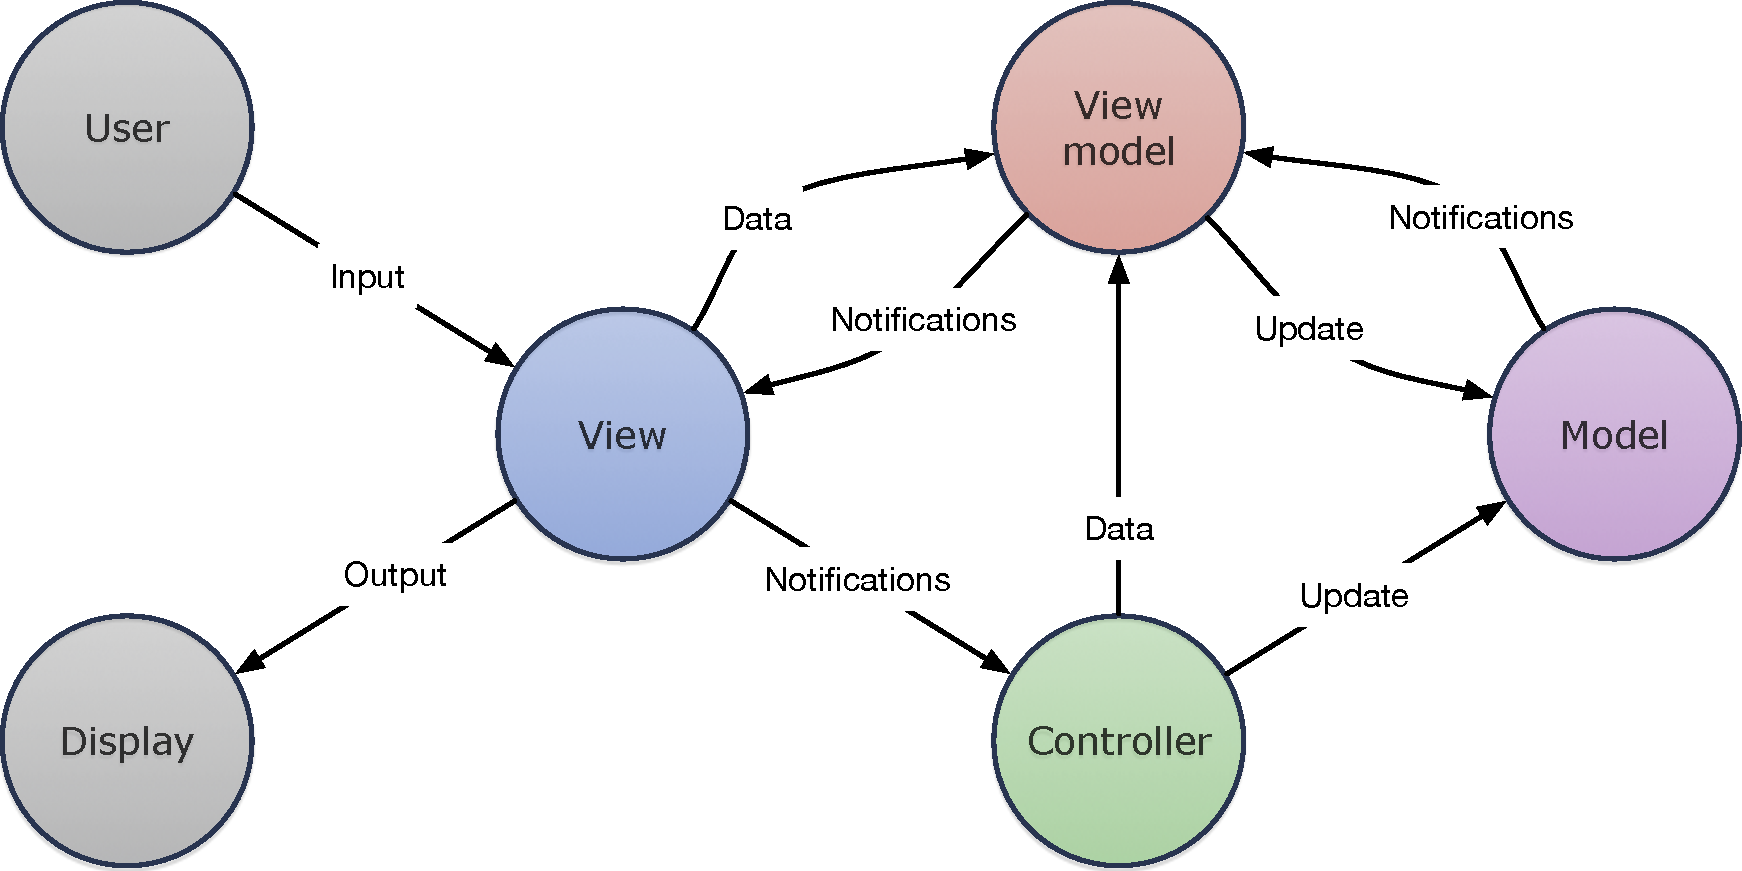
\includegraphics[width=0.8\linewidth]{images/mvvmc}
  \caption{Components of the used software design pattern and their communication.}
  \label{fig:software-design-pattern-components}
\end{figure}

\subsection{Software}

\newthought{The software itself} is an editor which allows \textit{modeling},
\textit{composing} and \textit{rendering} real time computer graphics through a
graphical toolbox. The editor was written in the python programming language
using the literate programming paradigm and uses the Qt framework as basis and
for the graphical user interface as well as OpenGL for rendering.

\newthought{Modeling} is done by composing single nodes to objects using a node
based graph structure. The basic nodes are defined by external files in JSON
notation. The graph structure allows adding, removing and connecting nodes to
complex objects. Every node has one ore more parameters, such as size or
position (of an object).

\newthought{Compositing} includes two aspects: the composition of objects into
scenes and the composition of an animation which is defined by multiple scenes
which follow a chronological order. The first aspect is realized by a scene
graph structure, which contains at least a root scene. Each scene may contain
objects in form of nodes which can be connected. The second aspect is realized
by a time line, which allows a chronological organization of scenes.

\newthought{For rendering} a highly optimized algorithm based on ray tracing is
used. The algorithm is called sphere tracing and allows the rendering of ray
traced scenes in real time on the GPU. Real-time means in this context being
able to generate at least 25 images in one second. Contingent upon the used
rendering algorithm all models are modeled using implicit surfaces.
% -*- mode: latex; coding: utf-8 -*-

\section{Conclusion and outlook}

\newthought{Literate programming takes some accustomization} as it requires a
different way of thinking to that of conventional software development. Despite
this, the basic goals could be reached. Sphere tracing is a very interesting and
promising approach to rendering which is coming into use in the industry, for
example for calculating ambient occlusion or soft shadows. Time will tell if the
method will establish itself further and become practicable for rendering
conventional meshes.

%\begin{figure}[h]
%\begin{center}
%\includegraphics[scale=0.45]{Roundabout.png}
%\caption{\small Roundabout maneuver 180$^o$ subdivided in pieces (1) to (9), with %several time- and speed indications.}
%\label{m2}
%\end{center}
%\end{figure}

% conference papers do not normally have an appendix

%% -*- mode: latex; coding: utf-8 -*-

% trigger a \newpage just before the given reference
% number - used to balance the columns on the last page
% adjust value as needed - may need to be readjusted if
% the document is modified later
%\IEEEtriggeratref{8}
% The "triggered" command can be changed if desired:
%\IEEEtriggercmd{\enlargethispage{-5in}}

% references section
% -*- mode: latex; coding: utf-8 -*-

% can use a bibliography generated by BibTeX as a .bbl file
% BibTeX documentation can be easily obtained at:
% http://mirror.ctan.org/biblio/bibtex/contrib/doc/
% The IEEEtran BibTeX style support page is at:
% http://www.michaelshell.org/tex/ieeetran/bibtex/
%\bibliographystyle{IEEEtran}
% argument is your BibTeX string definitions and bibliography database(s)
%\bibliography{IEEEabrv,../bib/paper}
%
% <OR> manually copy in the resultant .bbl file
% set second argument of \begin to the number of references
% (used to reserve space for the reference number labels box)
\printbibliography{}

% that's all folks
\end{document}
